\section{Krzysztof Wrona}

\subsection{Twierdzenie cosinusów}

To jest odniesienie do twierdzenia cosinusów - Figure \ref{fig:twierdzenie_cosinusow}

W dowolnym \textbf{trójkącie}, kwadrat długości dowolnego boku jest równy sumie kwadratów długości pozostałych boków pomniejszonej o \underline{podwojony} iloczyn długości tych boków i cosinusa kąta zawartego między nimi.

Zmiana z githuba

W szczególnym przypadku, gdy trójkąt jest prostokątny i $\gamma$ jest kątem prostym, twierdzenie to sprowadza się do twierdzenia Pitagorasa, ponieważ cosinus kąta prostego jest równy zeru


\[ c^2 = a^2 + b^2 - 2ab \cos \gamma \]


\begin{figure}[h] 
\centering
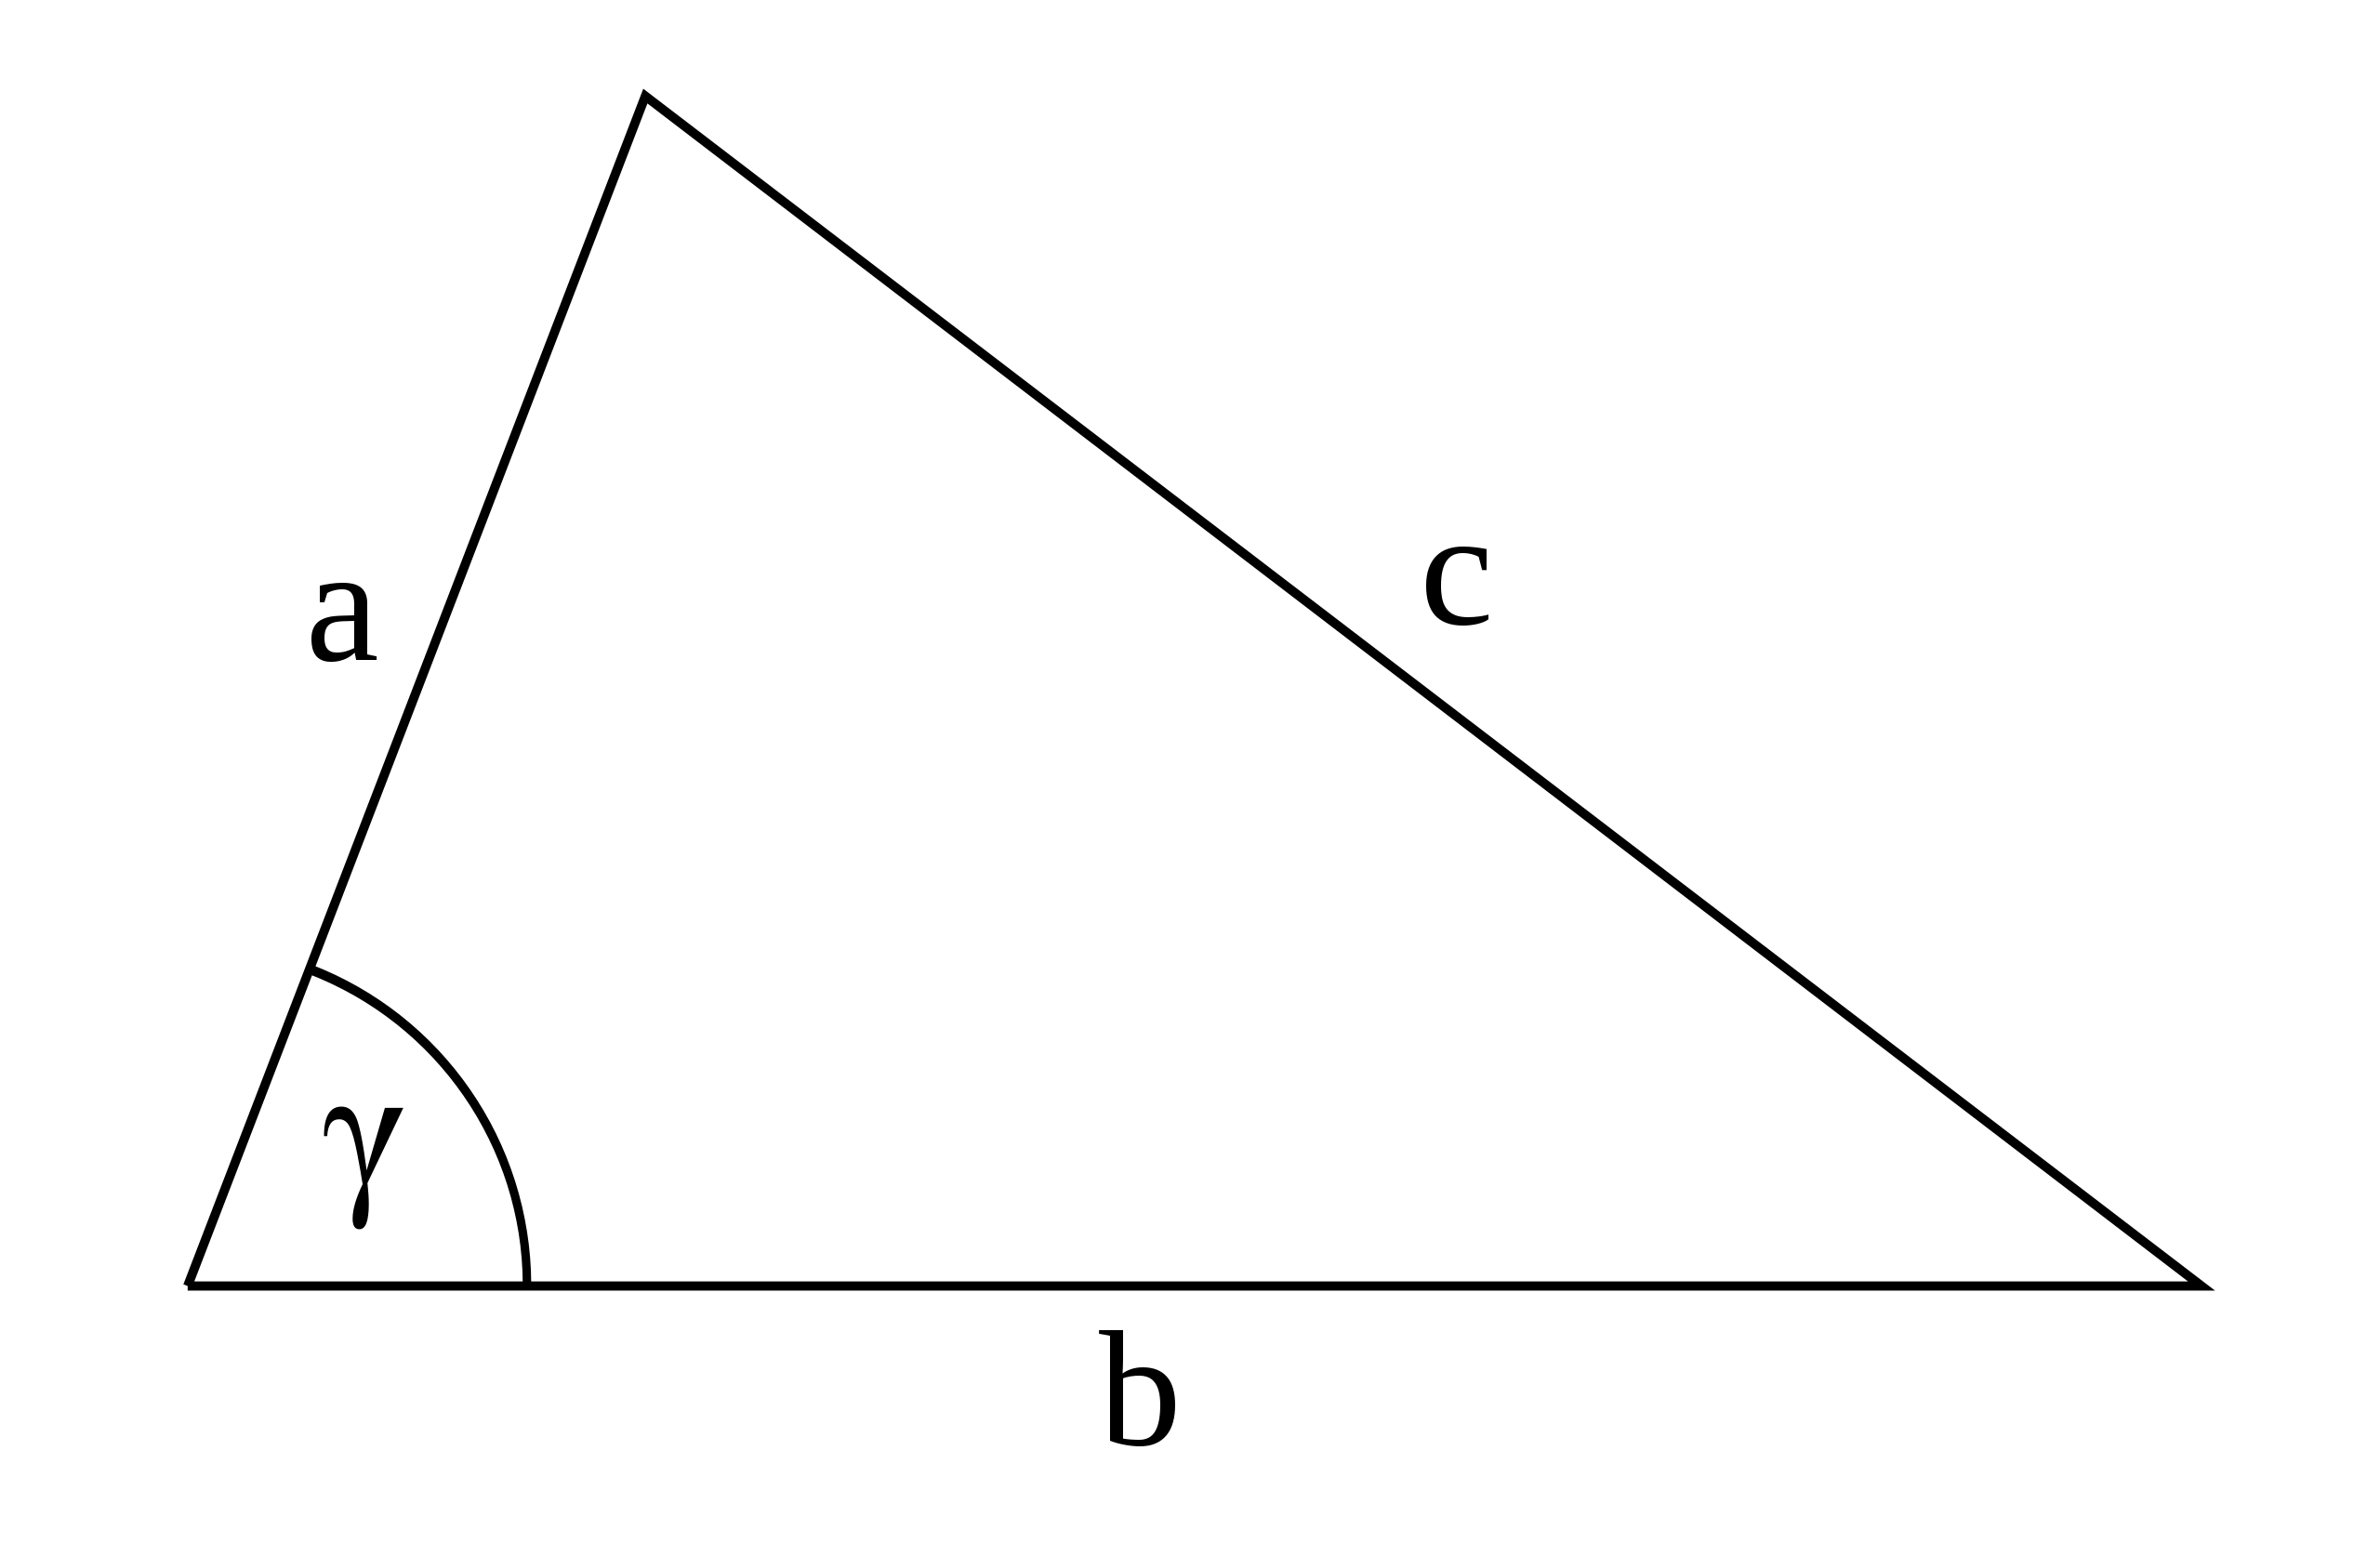
\includegraphics[width=0.6\textwidth]{pictures/twierdzenie_cosinusow.png}
\caption{\label{fig:twierdzenie_cosinusow}Twierdzenie cosinusów}
\end{figure}



\begin{table}[htbp]
\centering
\begin{tabular}{|c c c c|} 
 \hline
 a & b & c & $ \gamma $ \\ [0.5ex] 
 \hline\hline
 1 & 2 & 3 & 4 \\ 
 \hline
 10 & 20 & 30 & 40 \\
 \hline
 11 & 22 & 33 &  \\
 \hline
\end{tabular}
\label{tab:tabela4}
\caption{Przykładowe wartości}
\end{table}

\subsection{Zakupy}

Przykładowe listy zakupów

Owoce:

\begin{itemize}
\item jabłka
\item pomarańcze
\item banany
\item grejpfrut
\item cytryny
\end{itemize}

Warzywa:

\begin{enumerate}
\item cebula
\item ziemniaki
\item brokuły
\item marchew
\item buraki
\end{enumerate}
